% !TeX document-id = {1220ecc9-4e94-4765-8bf8-191a286a997a}
\documentclass[
	ngerman,
	parskip=half,
	twocolumn,
	DIV=calc,
	]{scrartcl}
	
\KOMAoptions{DIV=last}

\usepackage[utf8]{inputenc}
\usepackage[T1]{fontenc}

% Basic Look & Feel
\usepackage{babel}
\usepackage{lmodern}
\usepackage{microtype}
\usepackage{graphicx}
\usepackage{xspace}
\usepackage[xindy, nonumberlist, nogroupskip]{glossaries}
\usepackage{csquotes}
\usepackage{enumitem}
\usepackage{float}
\usepackage{gensymb, siunitx}
\sisetup{per-mode=symbol, binary-units=true}

% References
\usepackage[hyphens]{url}
\usepackage[hidelinks,linktoc=all]{hyperref}
\usepackage{cleveref}
\usepackage[backend=biber, style=ieee]{biblatex}
\addbibresource{bibliography.bib} 

% Tables
\usepackage{array}
\usepackage{booktabs}
\usepackage{multirow}

% Enable shell-escape
% !TeX TXS-program:compile = txs:///pdflatex/[--shell-escape]

%--------------------------------------------------------------------------------
%\lohead[]{}
%\rohead[]{\leftmark}
%\cohead[]{}

%
%captionsetup{format=plain,indention=2em}

%\makeglossaries
%\setacronymstyle{long-short}
%\loadglsentries{}

% Titel
\author{Sergej Zuyev}
\title{Projektarbeit}
\subtitle{Simuationsbasierter Entwurf eines A/D – Wandlers nach dem Prinzip des Integrationsverfahrens}
\subject{Schaltungstechnik SS2017}
\titlehead{
\includegraphics[width=\linewidth]{Logo_THM}}
\date{\today}

\graphicspath{{img/}}



%--------------------------------------------------------------------------------
\begin{document}
	
	\maketitle
	
	\pagenumbering{arabic}

	\clearpage
	
	\begin{abstract}		
	In diesem Dokument werden Modelle realer Operationsverstärker wie LT1800 und RC4558 untersucht und im Kontext der integrierenden Analog/Digital-Wandlung mit idealisierten Verstärkern verglichen.
	\end{abstract}
	
	\section{Einführung}	
	
		Im Rahmen der Veranstaltung \enquote{Elektronik 2 / Schaltungstechnik} bei Prof. Dr. Leitis wird zur Anerkennung als Prüfungsleistung das Thema \enquote{Integrierende Analog-Digital Wandler} behandelt.
		
		Hierbei wird das Verhalten der idealen Operationsverstärker (im Nachfolgendem OPAMP genannt) und realitätsnaher Modelle untersucht, insbesondere im Kontext der integrierierenden Analog/Digital Wandler.
	
	\section{Materialien und Methoden}
		\minisec{Simulationssoftware}
		
		Sämtliche Schaltungen wurden in SIMetrix\texttrademark 8.00p entwickelt,  simuliert, und für die finale Abgabe nach SIMetrix\texttrademark 5.60a portiert.
		Die Simulation wird ebenfalls in SIMetrix\texttrademark durchgeführt. 
		
		\minisec{Beurteilung}
		Eines der Hauptkriterien zur Beurteilung der Qualität eines A/D Wandlers ist das Quantisierungsrauschen: die Differenz zwischen dem Ein- und Ausgangssignal nach einer Rückwandlung in ein analoges Signal. 
		Dieses Kriterium wird näher betrachtet. 
		 
	\section{Ergebnisse}
		\subsection{Entwurf eines idealen Integrierers}
		\label{sec:ideal_integrator}
		Zunächst ist der Integrierer zu parametrisieren.		
		Die Ausgangsspannung berechnet sich wie folgt:
		
		\begin{equation}		
		V_c = \frac{1}{C}\int_{0}^{t_c} \frac{V_{in}}{R}dt
		\end{equation}
		
		Es ist eine Anstiegsrate von \SI{1}{\volt\per\milli\second} gefordert, somit sind die Zeit mit $t_c = \SI{1}{\milli\second} $ und die Spannung mit $V_{in} = \SI{1}{\volt}$ vorgegeben. Die Kapazität des Kondensators wird auf \SI{100}{\nano\farad} festgelegt, somit ist nur noch $R$ zu berechnen.
		
		Da $ V_{in} = \SI{1}{\volt} = const $ vereinfacht sich die obere Gleichung zu:		
		\begin{equation}
		V_c = \frac{V_{in}}{C \cdot R}t_c
		\end{equation}
		
		Nach der Auflösung nach $R$ werden die festgelegten Werte eingesetzt und der nötige Widerstand ermittelt: 
		\begin{equation}		
		R =  \frac{\SI{1}{\volt}}{\SI{100}{\nano\farad} \cdot \SI{1}{\volt}} \cdot \SI{1}{\milli\second} = \SI{10}{\kilo\ohm}
		\end{equation}
		
		
		Eine weitere Anforderung ist eine möglichst vollständige Idealisierung der in SIMetrix\texttrademark eingesetzten parametrisierbaren Operationsverstärker. 
		In \cref{tab:opamp-ideal-params} ist eine Zusammenstellung der wichtigsten Parameter aufgelistet. 
		
		In SIMetrix\texttrademark 5.60a führt der Ausgangswiderstand $R_{out} = 0$ während der transienten Analyse zu Konvergenzproblemen oder falschen Ergebnissen und ist somit unbrauchbar. Dasselbe gilt auch für GBWP in SIMetrix\texttrademark 8.00p.
		
		\begin{table}
			\centering
			\begin{tabular}{l c r r}
				\toprule
				\multirow{2}{*}{{Eigenschaft}}
					& \multirow{2}{*}{{Ideal}}
					& \multicolumn{2}{c}{{SIMetrix\texttrademark Version}} \\
					& & {8.00p} & {5.60a} \\
				\midrule
				CMRR & $\infty$ & $1G$ & $1G$ \\
				PSRR & $\infty$ & $1G$ & $1G$ \\
				Headroom & $0$ & $0V$ & $0V$\\
				Open-loop gain & $\infty$ &  $1G$ & $1G$\\
				GBWP & $\infty$ &  $3Meg$ & $1G$\\
				Slewrate & $\infty$ & $1G$ & $1G$ \\
				In. resistance & $\infty$ & $1G\Omega$ & $1G\Omega$ \\				
				Out. resistance & $0$ & $0\Omega$ & $100\Omega$\\
				In. bias current & $0$ & $0A$ & $0A$ \\
				In. offset voltage& $0$ & $0A$ & $0V$\\
				\bottomrule
			\end{tabular}		
		
			\caption{Ideale OPAMP Parameter}
			\label{tab:opamp-ideal-params}
		\end{table}
	
		\subsection{Entwurf von idealen integrierenden A/D-Wandlern}
		
		\minisec{Single-Slope A/D Wandler}
		\label{sec:single-slope-adc}		
	
		Der Integrator aus \cref{sec:ideal_integrator} wurde um eine Komparatorstufe und Steuerlogik erweitert, letztere ist aus einem \SI{9}{\bit} breiten Zähler und einem  \SI{8}{\bit} breiten Register zusammengesetzt. 
		Der Zähler ist auf einen Wertebereich von [0, 256] konfiguriert, und das 9-te Bit wird als Reset-Signal verwendet, welches die Entladung des Integrationskondensators initiiert.
		Der Komparator detektiert die Überschneidung zwischen $V_{in}$ und $V_{ref}$, und die unteren \SI{8}{\bit} des Zählers werden bis zum nächsten Auslösen ins Register übernommen.
		
		Der Eingangssignalbereich wird auf \SI{4}{\volt} Amplitude bei einem \SI{7}{\volt} Offset  festgelegt, und bei einer Auflösung von \SI{8}{\bit} berechnet sich die Taktperiode wie folgt: 
		
		\begin{equation}
		\label{eq:clock_period}
		T = \frac{\mid V_{max} - V_{min} \mid}{2^n  \cdot \SI{1}{\volt\per\milli\second}} = \frac{\SI{4}{\volt}}{2^8 \cdot \SI{1}{\volt\per\milli\second}} = \SI{15.625}{\volt\per\micro\second}	
		\end{equation}
				
		Mit der in \cref{eq:clock_period} berechneten Periodendauer ergibt sich die folgende skalierte Ansicht: 
		
		\begin{figure}[h!]
			\centering
			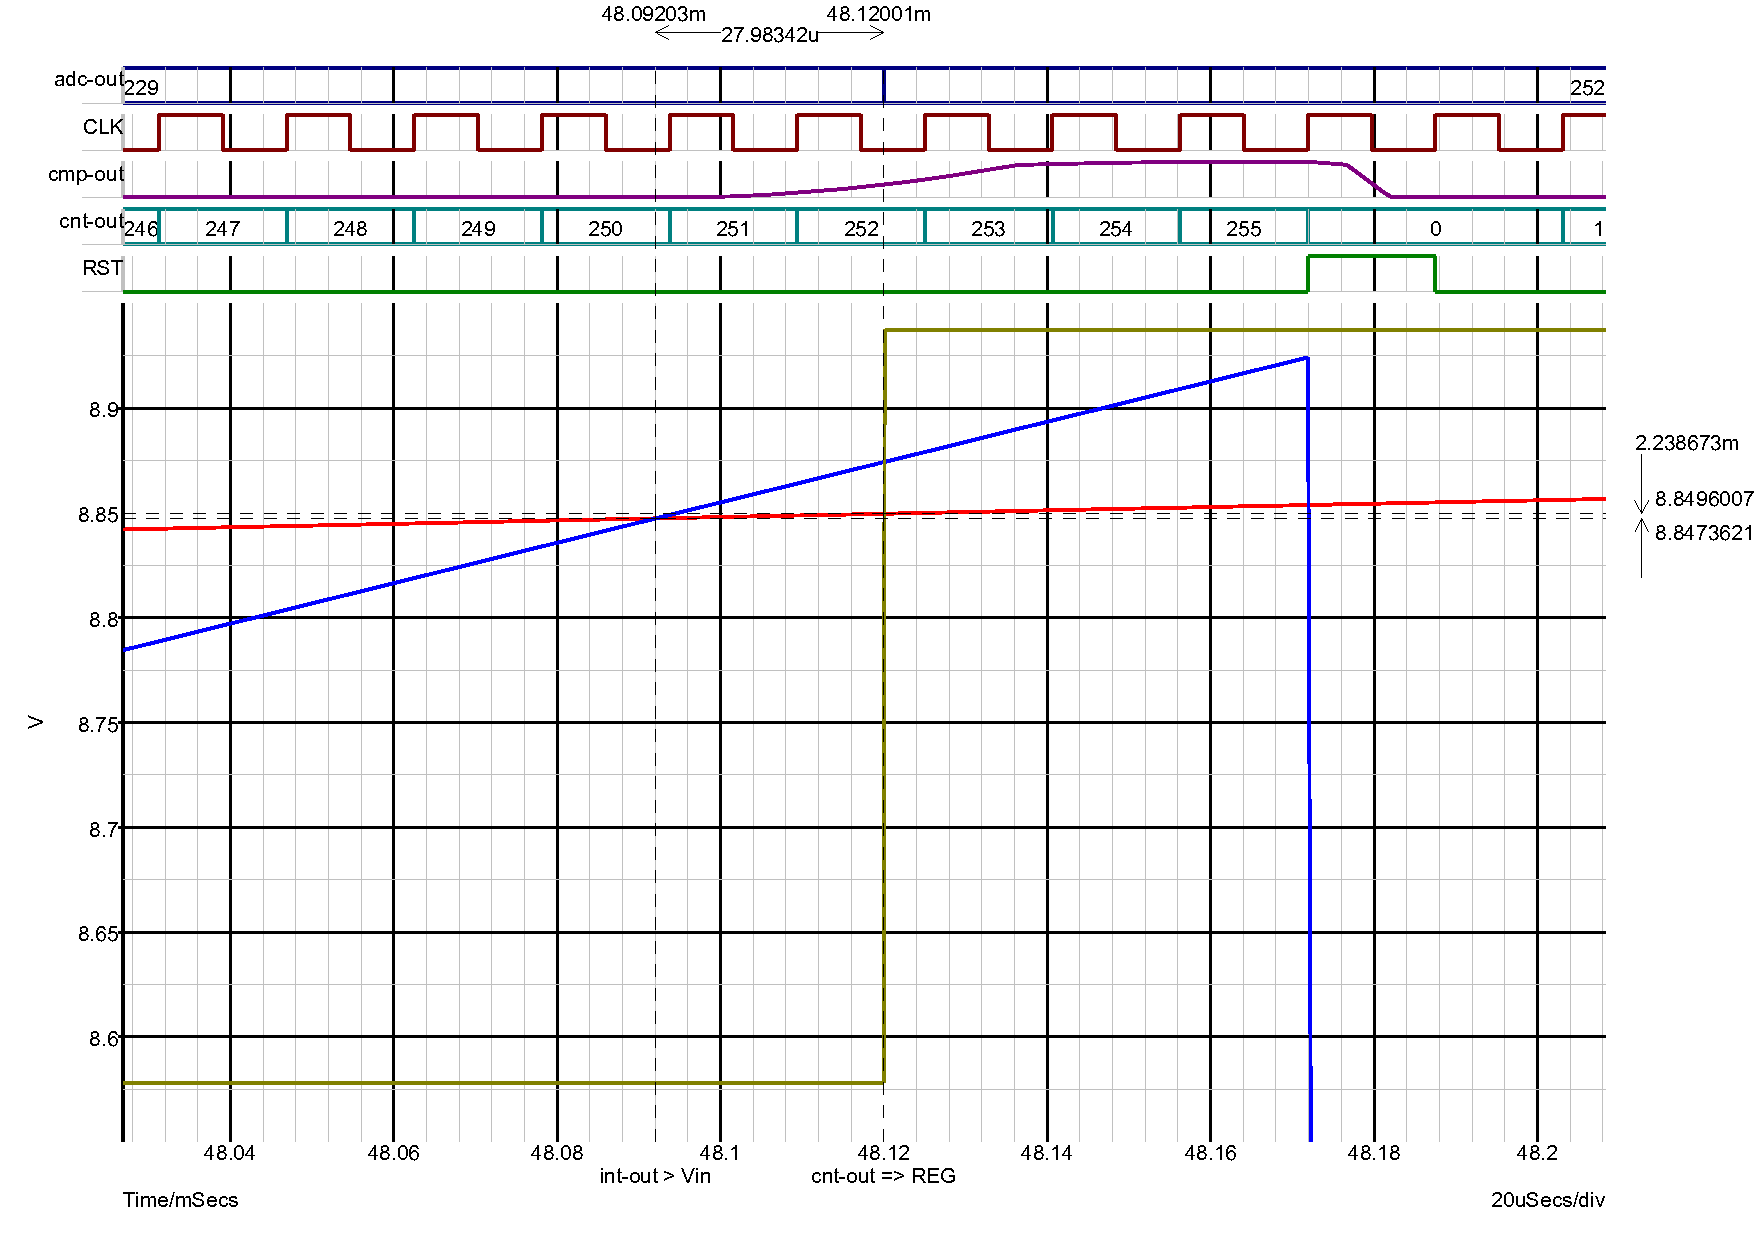
\includegraphics[width=\linewidth]{ideal_single_slope_odd_freq_comparator_slew_rate_wide}
			\caption[Single-slope ADC (T = \SI{15.625}{\micro\second})]{Single-slope ADC, $T \Rightarrow \SI{15.625}{\micro\second}$, $V_{in} \Rightarrow [5,  9]$}
			\label{fig:single-slope-ideal-slew-rate}
		\end{figure}	
	
		Man kann deutlich erkennen, dass unter diesen Bedingungen der Integrationsprozess nicht abgeschlossen ist, da die \SI{9}{\volt} Soll nicht erreicht sind, und dass sich aufgrund der Slew-Rate des Komparators das Signal zur Aufnahme des Zählerstandes sich um einen Takt verzögert. Dies führt zur Übernahme des inkrementierten Zählerstandes, das Ausgangssignal weist einen Offset nach oben auf und das Quantisierungsrauschen steigt.
		
		Wenn man die Periodendauer auf \SI{16}{\micro\second} aufrundet, erhält man, wie auf \cref{fig:single-slope-ideal} zu sehen ist, ein wesentlich besseres Ausgangssignal, und das Quantisierungsrauschen beträgt nahezu 0 für jedes neue Sample. 
		
		\begin{figure}[h!]
			\centering
			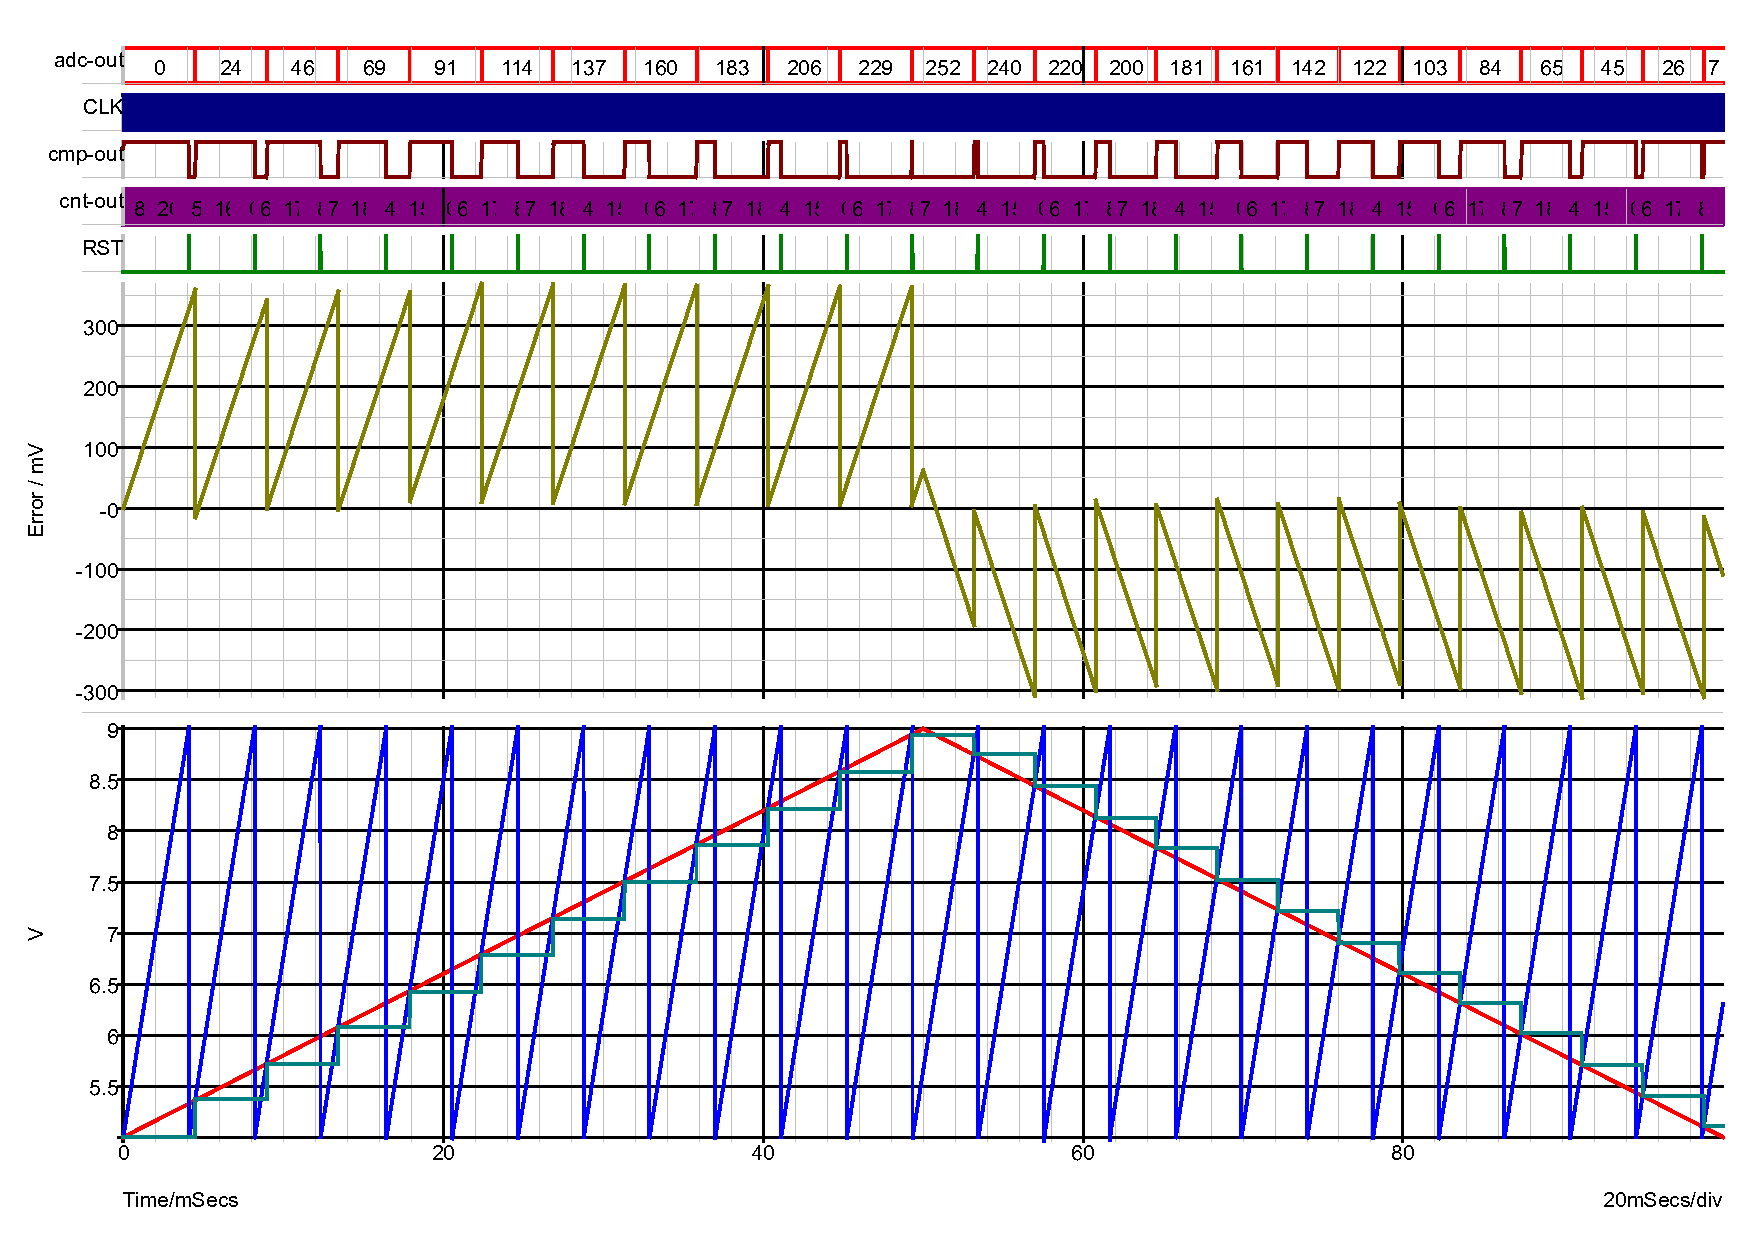
\includegraphics[width=\linewidth]{ideal_single_slope}
			\caption[Single-slope ADC (T = \SI{16}{\micro\second})]{Single-slope ADC, $T \Rightarrow \SI{16}{\micro\second}$, $V_{in} \Rightarrow [5,  9]$}
			\label{fig:single-slope-ideal}
		\end{figure}
		
		
		\minisec{Dual-Slope A/D Wandler}
		\label{sec:dual-slope-adc}
		
		Aufbauend auf dem single-slope Wandler aus dem vorhergehendem Kapitel wird die Steuerlogik angepasst: der Zähler wird auf \SI{10}{\bit} mit einem Wertebereich von [0, 512] erweitert. Bit 9 signalisiert nun die Deintegrationsphase, Bit 10 wird als Reset-Signal verwendet.
				
		Zusäzlich wurden ein Eingangsmultiplexer, um zwischen $V_{ref} $und $V_{in} $ umzuschalten, und ein Unity-Gain-Buffer verbaut.
		Wird an diesen nun $V_{ref} $ geschaltet, so wird das SIgnal 1:1 am Integrierer anliegen. Dem $V_{in}$ Eingang ist allerdings ein \SI{3}{\kilo\ohm} Widerstand nachgeschaltet, dadurch agiert der  Spannungsfolger als Dämpfer mit einem Verstärkungsfaktor $ A = \frac{\SI{1}{\kilo\ohm}}{\SI{3}{\kilo\ohm} + \SI{1}{\kilo\ohm}} = \frac{1}{4}$ und passt den Bereich von $V_{in} $ auf $V_{ref} $ an. Somit ist eine konstante De- und Integrationsrate von \SI{1}{\volt\per\micro\second} gewährleistet.
		
		Da von nun an eine Auswertung des Integrators nur noch jeden zweiten Takt erfolgt, führt das zu Halbierung der Abtastrate und somit dem Nyquist-Theorem entsprechend zur Halbierung der möglichen Eingangsfrequenz - das kann man auf \cref{fig:dual-slope-ideal} gut erkennen, trotz gleicher Taktung werden ungefähr halb so viele Samples aufgenommen. Darüber hinaus macht sich ein zum Eingangssignal proportionaler Quantisierungsfehler bemerkbar, dieser ist mit dem Quantisierungsrauschen überlagert.
		
		\begin{figure}
			\centering
			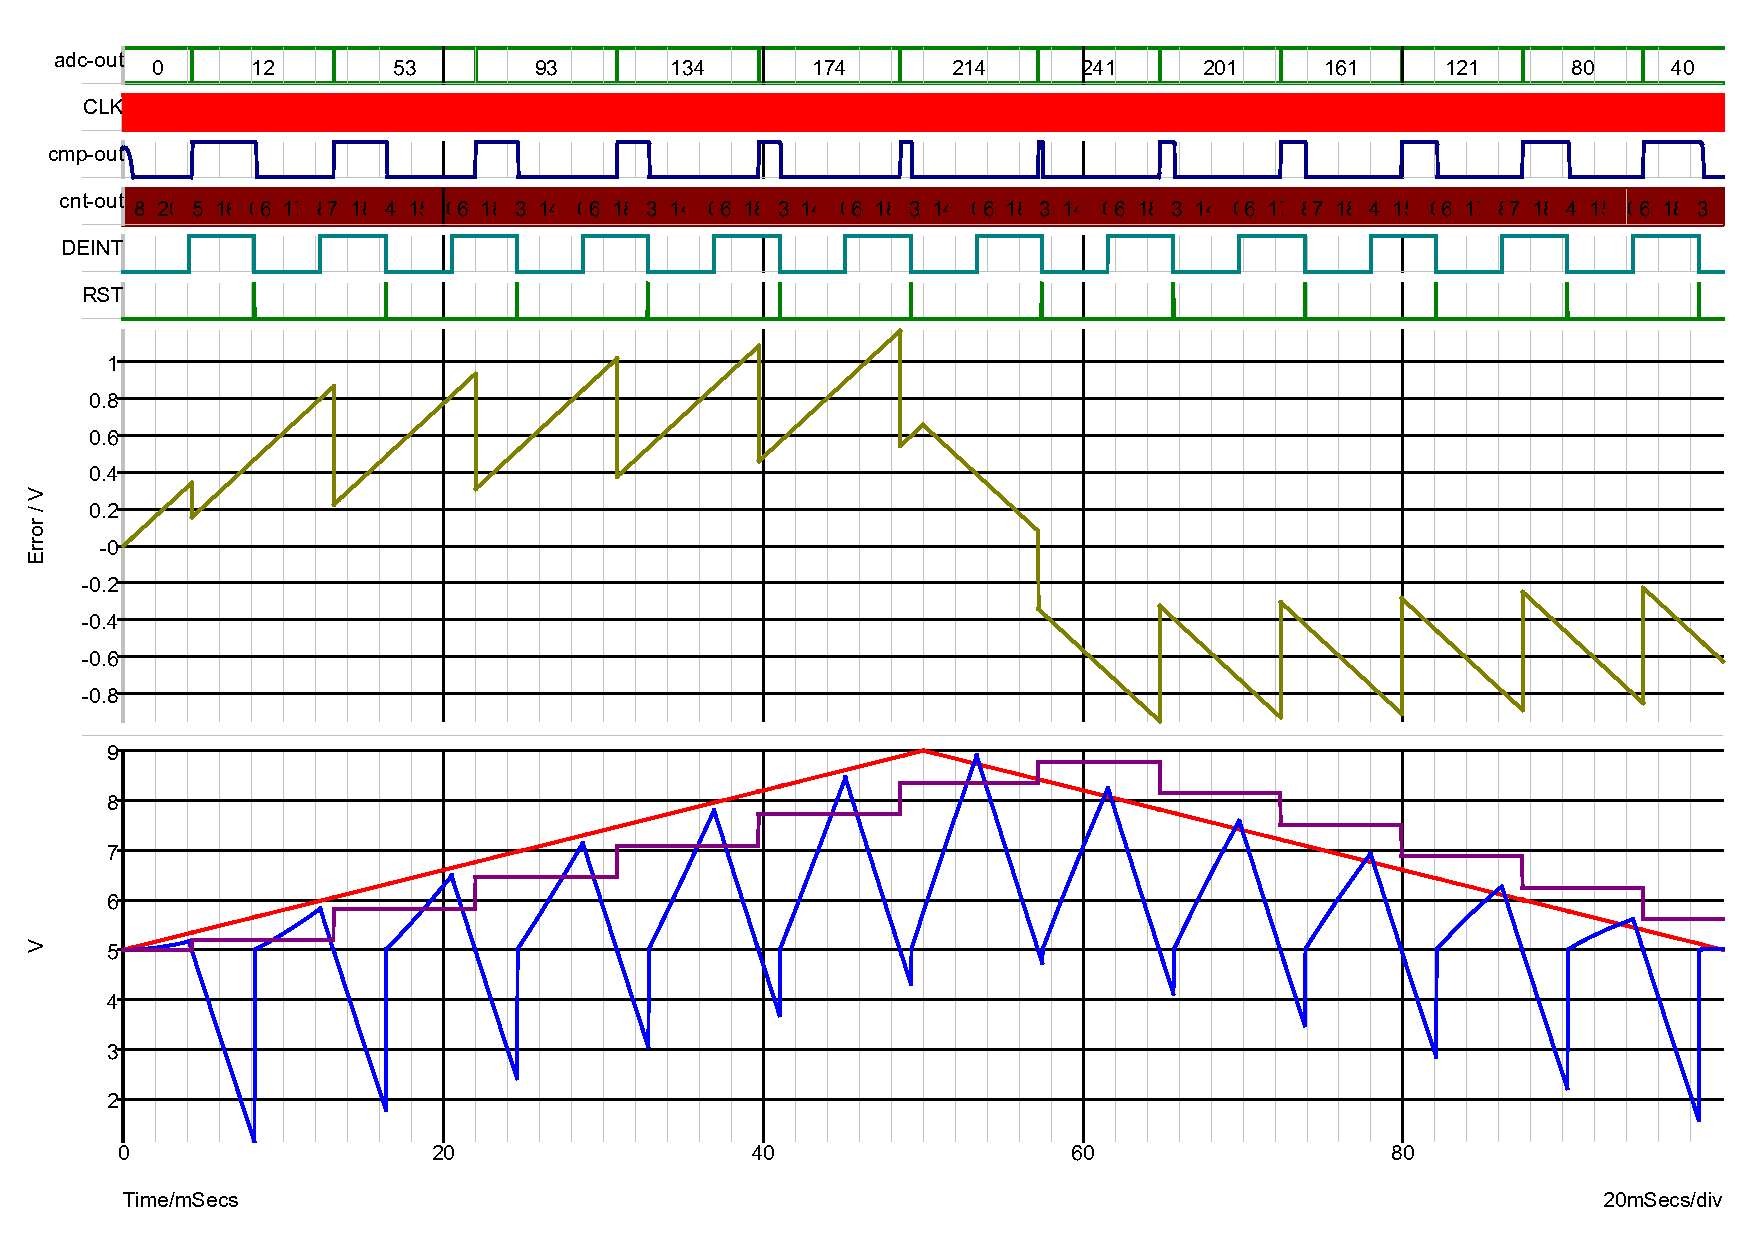
\includegraphics[width=\linewidth]{ideal_dual_slope}
			\caption[Dual-slope ADC]{Dual-slope ADC, $T \Rightarrow \SI{16}{\micro\second}$, $V_{in} \Rightarrow [5,  9]$}
			\label{fig:dual-slope-ideal}
		\end{figure}
	
		\subsection{Analyse des RC4558 Modells}
		\label{sec:opamp_analysis}		
		
		Während der Integration des LT1800 OPAMP-Modells in die single-slope und dual-slope Wandler ist ein unerwartetes Problem aufgetreten: 
		die Anzahl der Analogknoten ist in der frei erhältlichen SIMetrix\texttrademark Version limitiert. Nachweislich überschreitet der Einsatz zweier und mehr Operationsverstärker des Typs LT1800  die Simulationsbeschränkungen, wie der Datei \enquote{zuyev\_1.4\_LT1800 - dual slope adc.sxsch} zu entnehmen ist. Darum wird im Nachfolgendem der OPAMP RC4558 von Texas Instruments untersucht. Die Analyse des LT1800-Modells ist im \cref{sec:appendix_LT1800_analysis} zu finden.		
	
		Der RC4558 ist ein universeller Verstärker ohne Rail-To-Rail-Verhalten und wird für den Einsatz als Spannungsfolger empfohlen. 
		Die Versorgungsspannung darf maximal $ \pm\SI{18}{\volt} $ betragen, empfohlen werden $ \pm5-\pm\SI{15}{\volt}$. Somit ist dieser nicht für den unipolaren Betrieb geeignet.
		
		Bei der Simulation ergibt sich eine gute Übereinstimmung des Modells mit den Kenndaten \cite{datasheet:RC4558}. Besondere Aufmerksamkeit im Vergleich zum LT1800 verdienen die vergleichsweise niedrigen Slew-Rate und Gain-Bandbreite: Nach 3MHz ist der Unity-Gain-Pol erreicht, und aufgrund der niedrigen Slew-Rate kann bei hohen Frequenzen nicht die volle Ausgangsspannung erreicht werden. Diese Daten entsprechen der grundsätzlichen Empfehlung zur Verwendung als Spannungsfolger. 
		
		Die Gegenüberstellung der Simulationsergebnisse und der typischen Werte aus dem Datenblatt \cite{datasheet:RC4558} lässt sich aus \cref{tab:opamp-RC4558} entnehmen. 
	
		\begin{table}[h!]
			\centering
			\begin{tabular}{l r r}
				\toprule				
				\multirow{2}{*}{Eigenschaft} &
					\multicolumn{2}{c}{Wert} \\
					& Simuliert & Datenblatt \cite{datasheet:RC4558} \\
				\midrule
				
				V\textsubscript{os} 											& $ \approx \SI{9.4}{\micro\volt}  $ &  0.5--\SI{6}{\milli\volt}  \\			
				I\textsubscript{bias} 											 & $ \approx-139.56$ 		& 150--\SI{800}{\nano\ampere}  \\			
				V\textsubscript{swing} 										  & $ \approx\pm9.8$ 		 & $ \pm \SI{10}{\volt} $ \\
				 $A_{VOL}$														   & $\approx \SI{70}{\decibel}$ 		   & N/A \\
				CMRR 																  & $\approx78.4$ 		      & 70--\SI{90}{\decibel}\\
				PSRR  																   & $\approx \SI{99.8}{\decibel}$ 		   & N/A \\
				SR 																		 & $ \approx 1.809$ 		 & 1.1--\SI{1.7}{\volt\per\micro\second}\\
				GBWP 															     & $\approx 3.09$ 			  & \SI{3}{\mega\hertz}\\
				\bottomrule
			\end{tabular}
			\caption[RC4558 Parameter]{RC4558 Parameter, $V \Rightarrow \pm \SI{15}{\volt}, T_A \Rightarrow  \SI{25}{\celsius}  $}
			\label{tab:opamp-RC4558}
		\end{table}
	
		\subsection{Entwurf der integrierenden A/D-Wandler mit Modellen realer Komponenten}		
		
		Wie im \cref{sec:opamp_analysis} bereits erwähnt, ist der RC4558 nicht für den unipolaren Betrieb geeignet. Deshalb kann die Anforderung, alle Schaltungen unipolar zu betreiben, in diesem Fall nicht erfüllt werden. 
		
		Die Versorgungsspannung wurde vorsichtshalber auf $\pm \SI{15}{\volt} $ erhöht, da dieser OpAmp kein Rail-To-Rail Verstärker ist und bis zu $\pm \SI{2}{\volt} $ Headroom aufweist. 
		
		Die Abtastrate konnte für beide Wandler-Variationen verfünffacht werden, weitere Erhöhung über den Faktor 5 hinaus führte zunächst zu einer Steigerung des Quantisierungsrauschens und im Anschluss zum Versagen - aufgrund der niedrigen Slew-Rate und zu hohen Frequenz werden wie in \cref{sec:single-slope-adc} beschrieben falsche Werte ermittelt. 
		
		Auffällig ist der Verlauf des Quantisierungsrauschens im Vergleich zu den niedriger getakteten Pendants aus \cref{sec:single-slope-adc}: Im Falle des single-slope Wandlers, verändert sich der Verlauf sehr stark, wie in \cref{fig:single-slope-RC4558} zu sehen ist, und weist einen zum Eingangssignal proportionalen Quantisierungsfehler auf, ähnlich wie der idealisierte dual-slope Wandler.				
				
		\begin{figure}
			\centering
			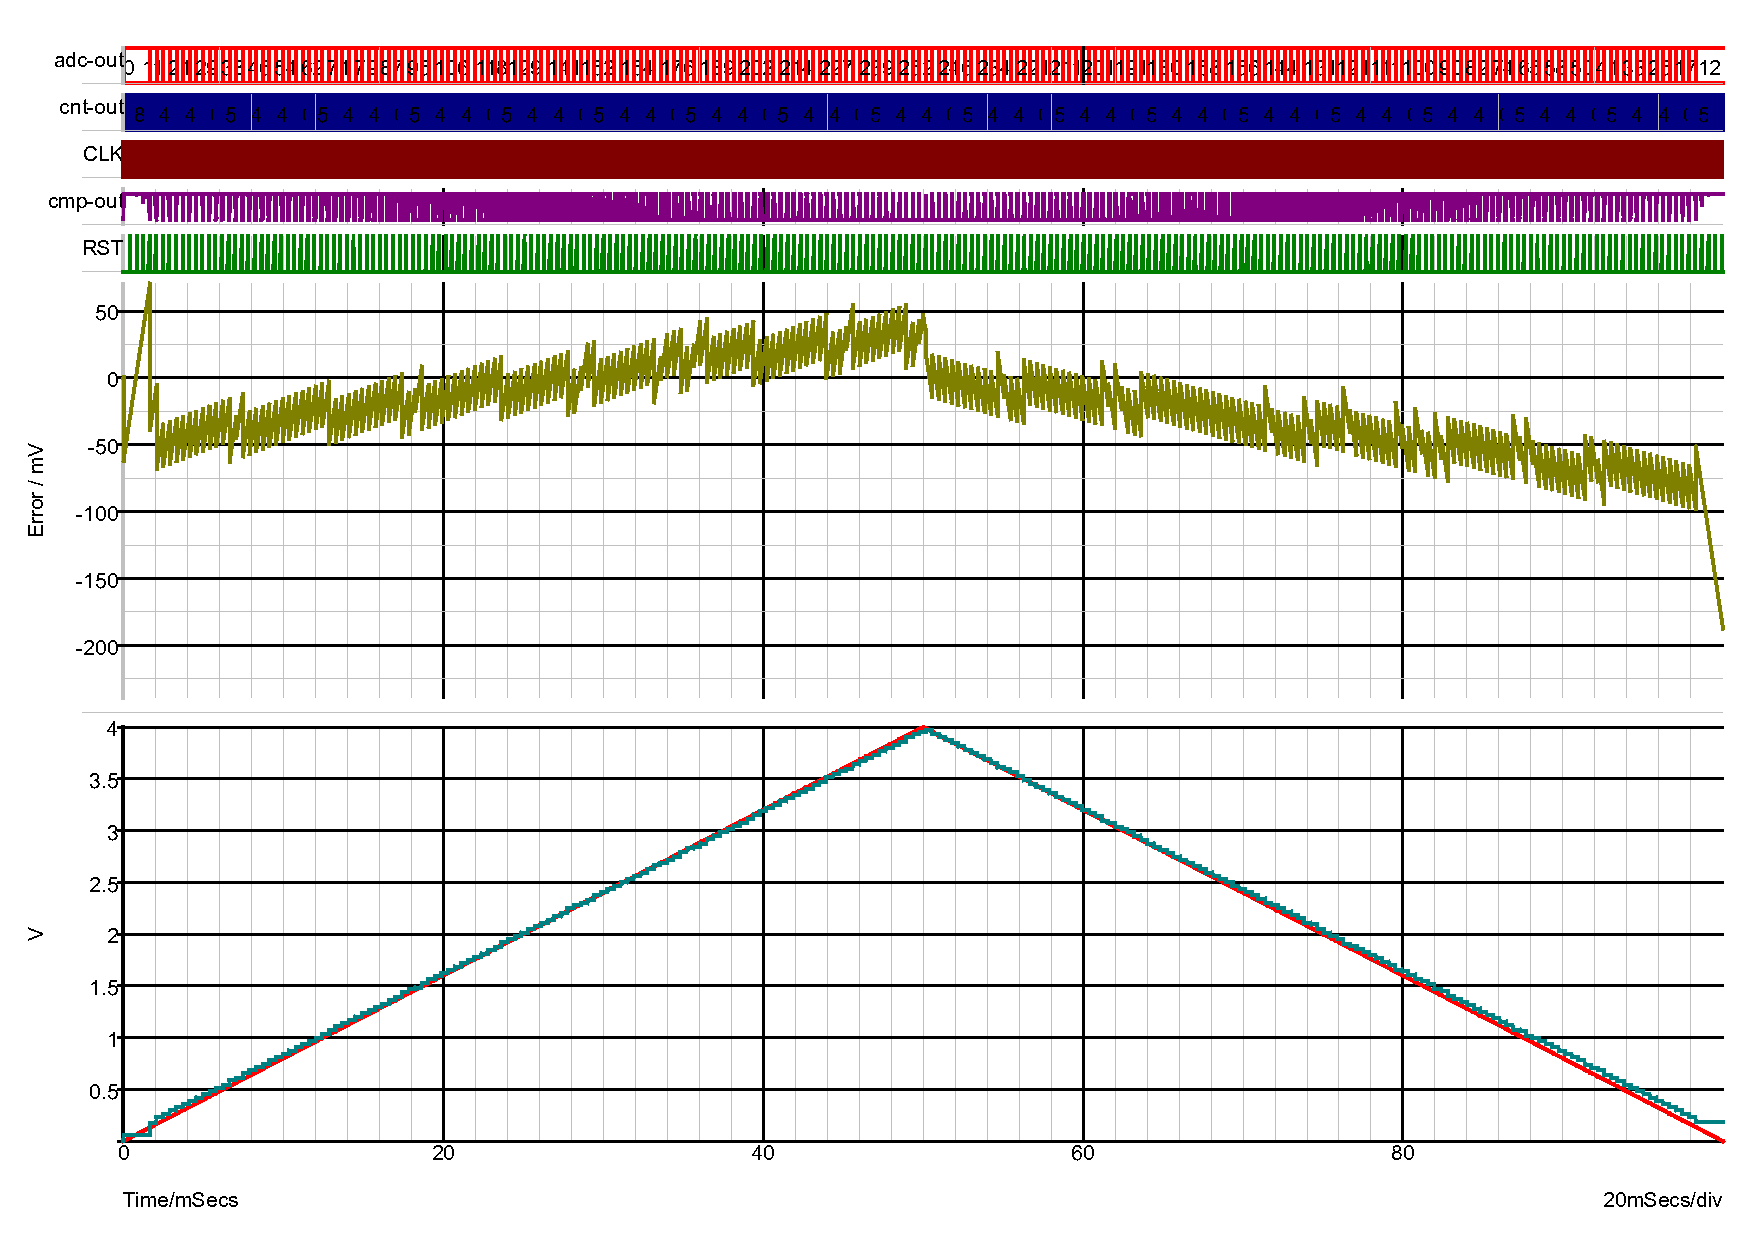
\includegraphics[width=\linewidth]{RC4558_single_slope}
			\caption[Single-slope RC4558 ADC]{Single-slope RC4558 ADC, $T \Rightarrow 1.6\mu s$, $V_{in} \Rightarrow [5,  9]$}
			\label{fig:single-slope-RC4558}
		\end{figure}	
	
		Der dual-slope Wandler hingegen weist, abgesehen vom Offset und der höheren Frequenz, ein zur idealisierten Variante nahezu unverändertes Quantisierungsrauschen auf. Dieses ist in \cref{fig:dual-slope-RC4558} dargestellt.
	
		\begin{figure}
			\centering
			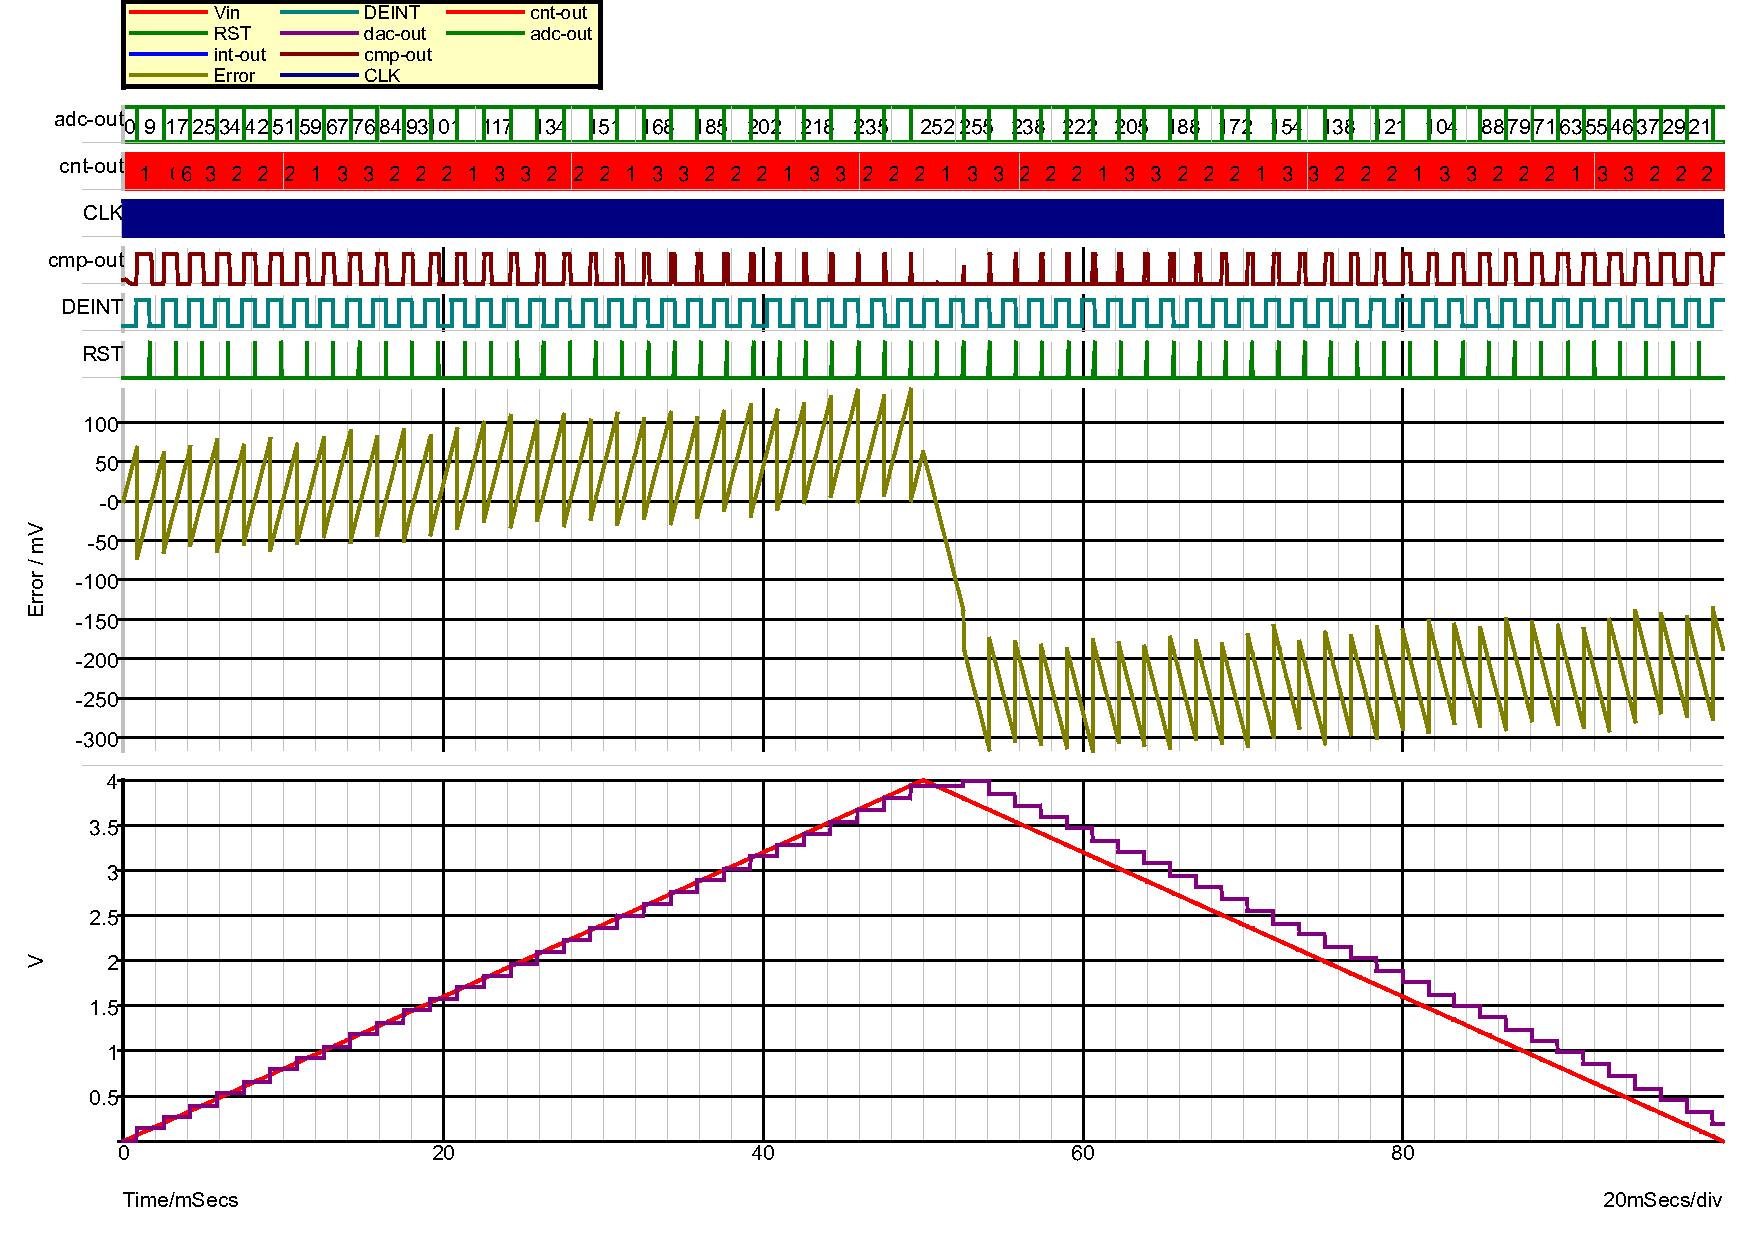
\includegraphics[width=\linewidth]{RC4558_dual_slope}			
			\caption[Dual-slope RC4558 ADC]{Dual-slope RC4558 ADC, $T \Rightarrow 3.2\mu s$, $V_{in} \Rightarrow [5,  9]$}			
			\label{fig:dual-slope-RC4558}
		\end{figure}
	\section{Fazit}	
		Im Aufbau mit idealisierten Komponenten verhält sich der single-slope Wandler wesentlich besser als der dual-slope Wandler: Das Quantisierungsrauschen  ist niedriger, und die Abtastrate ist doppelt so hoch. Simuliert man allerdings mit Modellen realer Komponenten, so kehrt sich die Situation um. Daraus werden die Vorteile eines dual-slope-ADC ersichtlich, nämlich die Kompensation möglicher Komponententoleranzen durch einen Deintegrationsschritt.
		
		Der Aufbau behandelt keine Überschreitung der Eingangsspannung.  Dies hat eine Aufnahme zu niedriger Werte zur Folge. Denkbar wäre es, beim Überlauf des Zählers den Maximalwert ins Register zu übernehmen, falls der Komparator keine Überschneidung signalisiert hat. 
		
		Den Komparatorausgang direkt als Clock-Eingang für das Register zu verwenden kann gefährlich sein, da die Ausgangsspannung durchaus prellen könnte (Slew-Rate Überschwinger). Mäglich wäre es, den Komparator um einen Schmitt-Trigger\cite{website:schmitt_trigger_slewrate} mit einer zur Abtastfrequenz passenden Hysterese zu erweitern bzw umzuwandeln.
		
	\section{Anhang}
	
	\subsection{Analyse des LT1800 Modells}
	\label{sec:appendix_LT1800_analysis}
	Der LT1800 ist ein Präzisionsverstärker, hat einen Rail-To-Rail Ein- und Ausgang, und ist insbesondere für Signalverarbeitung gedacht, dazu gehören auch A/D Wandler. Die zulässige Versorgungsspannung liegt zwischen \SI{2.3}{\volt} und \SI{12.6}{\volt}, jedoch werden nur 3 Bereiche empfohlen: 0--\SI{3}{\volt}, 0--\SI{5}{\volt}  und $\pm\SI{5}{\volt} $. Die Simulation ergab vielversprechende Ergebnisse, diese entsprechen weitestgehend dem Datenblatt \cite{datasheet:LT1800}, wie in \cref{tab:opamp-LT1800}  dargestellt.
	
	\begin{table}[h!]
		\centering
		\begin{tabular}{l l r r}
			\toprule
			\multirow{2}{*}{Eigenschaft} & \multirow{2}{*}{Bedingung} &
			\multicolumn{2}{c}{Wert} \\
			&& Simuliert & Datenblatt \cite{datasheet:LT1800} \\
			\midrule		
			
			$V_{os}$											  			     && $ \approx  \SI{241.85}{\micro\volt} $ & \SI{150}{\micro\volt}--\SI{0.7}{\milli\volt} \\			
			$I_{bias}$					          &$V_{cm} = \SI{1}{\volt}$ & $\approx -2.39$         & 25--\SI{350}{\nano\ampere} \\			
			$I_{bias}$ 					  		 & $V_{cm} = V_{s}$	   & $\approx 547.4$         & 400--\SI{1500}{\nano\ampere} \\		
			$V_{swing low}	 $		 & $I = 0mA$& $ \approx 13 $ 			& 12--\SI{50}{\milli\volt}  \\ 
			$V_{swing high} $		 &	$ I = 0mA$& $ \approx 22 $    		& 16--\SI{60}{\milli\volt} \\
			$V_{swing low}  $		 &$ I = 5mA$	& $  \approx 12.9$   & 80--\SI{160}{\milli\volt}    \\ 
			$V_{swing high}$		 & $I = 5mA$ & $ \approx   80.1$   & 120--\SI{250}{\milli\volt}   \\
		    $V_{swing low}$		& $I = 20mA$ & $  \approx  12.9 $   & 225--\SI{450}{\milli\volt}    \\ 
			$V_{swing high}$		& $ I = 20mA$ & $ \approx   249 $   & 450--\SI{850}{\milli\volt}  \\
		    $A_{VOL}$					&									  & $\approx 98.5 $				& 35--\SI{85}{\decibel} \\
			CMRR 							&									   & $\approx 85.8$ 		  & 85--\SI{105}{\decibel}\\
			PSRR 							&										& $\approx 86.2$ 			& 80--\SI{97}{\decibel} \\
			SR 									&									  & $ \approx 24.3 $ 		& 13--\SI{25}{\volt\per\micro\second}\\
			GBWP 							&									  & $\approx 90.1$ 				& 40--\SI{80}{\mega\hertz}\\
			\bottomrule
		\end{tabular}
		\caption[LT1800 Parameter]{LT1800 Parameter, $V \Rightarrow 5-0V, T_A \Rightarrow  \SI{25}{\celsius}  $}
		\label{tab:opamp-LT1800}
	\end{table}

	\subsection{Messverfahren RC4558}
	\label{sec:appendix_measurement_methods_RC4558}
	Zur besseren Nachvollziehbarkeit der Ergebnisse folgt in diesem Kapitel eine Beschreibung der notwendigen Simulationsschritte. 	
	\minisec{Slew rate}	
	Datei: \emph{RC4558 - slew rate}
	\begin{enumerate}
		\item Die Kurve \enquote{VOut} auswählen
		\item Measure $\rightarrow$ More Functions... $\rightarrow$ Rise Time 10\%-90\% (auto)
		\item $SR = \SI{500}{\milli\volt} \cdot 80\% \cdot \frac{\SI{1}{\micro\second}}{t_{rise}}$
	\end{enumerate}

	\minisec{Input bias current}
	Datei: \emph{RC4558 - input bias current}
	\begin{enumerate}
		\item Die Kurve \enquote{I(bias)} auswählen
		\item Measure $\rightarrow$ Mean
	\end{enumerate}

	\minisec{Input offset voltage}	
	Datei: \emph{RC4558 - voffset}
	
	Hier wurde ein erweitertes Messverfahren \cite{website:amp_psrr_cmrr_circuits} verwendet.
	\begin{enumerate}
		\item Die Kurve \enquote{VOffset} auswählen
		\item Measure $\rightarrow$ Mean
	\end{enumerate}

	\minisec{CMRR}	
	Datei: \emph{RC4558 - cmrr}
	
	Hier wurde ein erweitertes Messverfahren \cite{website:amp_psrr_cmrr_circuits} verwendet.
	\begin{enumerate}
		\item Die Kurven $V_{cm}$ und $V_{offset}$ auswählen.
		\item Measure $\rightarrow$ More Functions... $\rightarrow$ Peak To Peak $\Rightarrow 2\hat{V}_{cm}$
		\item $ CMRR = 20 * log_{10} \frac{2\hat{V}_{cm}}{2\hat{V}_{offset}}$
	\end{enumerate}

	\minisec{PSRR}	
	Datei: \emph{RC4558 - psrr}
	
	Hier wurde ein erweitertes Messverfahren \cite{website:amp_psrr_cmrr_circuits} verwendet.
	\begin{enumerate}
		\item Die Kurven $V_{dd}$ und $V_{offset}$ auswählen.
		\item Measure $\rightarrow$ More Functions... $\rightarrow$ Peak To Peak $\Rightarrow 2\hat{V}_{dd}$
		\item $ PSRR = 20 * log_{10} \frac{2\hat{V}_{dd}}{2\hat{V}_{offset}}$
	\end{enumerate}

	\minisec{Open loop gain}	
	Datei: \emph{RC4558 - olgain}
	
	Hier wurde ein erweitertes Messverfahren \cite{website:amp_psrr_cmrr_circuits} verwendet.
	\begin{enumerate}
		\item Die Kurve $Gain$ auswählen.
		\item Measure $\rightarrow$ Maximum
	\end{enumerate}
	

	\minisec{Gain bandwidth product}
	Datei: \emph{RC4558 - unity gain bandwidth}
	\begin{enumerate}
		\item Die Kurve $Gain$ auswählen
		\item Measure $\rightarrow$ More Functions... $\rightarrow$ Lowpass \SI{-3}{\decibel} (db Plot, auto) $\Rightarrow f_{3dB}$
		\item $ GBP = A \cdot f_{3dB} = 10 \cdot f_{3dB} $
	\end{enumerate}

	\minisec{Voltage swing}	
	Datei: \emph{RC4558 - voltage swing}
	\begin{enumerate}
		\item Die Kurven $V_{out RL=100G}$, $V_{out RL=10k}$, $V_{out RL=2k}$ auswählen. $R_L=\SI{100}{\giga\ohm}$ simuliert den Leerlauf.
		\item Measure $\rightarrow$ More Functions... $\rightarrow$ Peak To Peak $\Rightarrow 2\hat{V}$
		\item $V_{swing} = \pm \frac{2\hat{V}}{2}$
	\end{enumerate}

	\subsection{Messverfahren LT1800}
	\label{sec:appendix_measurement_methods_LT1800}
	Zur besseren Nachvollziehbarkeit der Ergebnisse folgt in diesem Kapitel eine Beschreibung der notwendigen Simulationsschritte. 	
	\minisec{Slew rate}	
	Datei: \emph{LT1800 - slew rate}
	\begin{enumerate}
		\item Die Kurve \enquote{VOut} auswählen
		\item Measure $\rightarrow$ More Functions... $\rightarrow$ Rise Time 10\%-90\% (auto)
		\item $SR = \SI{3}{\volt} \cdot 80\% \cdot \frac{\SI{1}{\micro\second}}{t_{rise}}$
	\end{enumerate}
	
	\minisec{Input bias current}
	Datei: \emph{LT1800 - input bias current}
	\begin{enumerate}
		\item Die Kurven \enquote{I(bias)} auswählen
		\item Measure $\rightarrow$ Mean
	\end{enumerate}
	
	\minisec{Input offset voltage}	
	Datei: \emph{LT1800 - voffset}
	
	Hier wurde ein erweitertes Messverfahren \cite{website:amp_psrr_cmrr_circuits} verwendet.
	\begin{enumerate}
		\item Die Kurve \enquote{VOffset} auswählen
		\item Measure $\rightarrow$ Mean
	\end{enumerate}
	
	\minisec{CMRR}	
	Datei: \emph{LT1800 - cmrr}
	
	Hier wurde ein erweitertes Messverfahren \cite{website:amp_psrr_cmrr_circuits} verwendet.
	\begin{enumerate}
		\item Die Kurven $V_{cm}$ und $V_{offset}$ auswählen.
		\item Measure $\rightarrow$ More Functions... $\rightarrow$ Peak To Peak $\Rightarrow 2\hat{V}_{cm}$
		\item $ CMRR = 20 * log_{10} \frac{2\hat{V}_{cm}}{2\hat{V}_{offset}}$
	\end{enumerate}
	
	\minisec{PSRR}	
	Datei: \emph{LT1800 - psrr}
	
	Hier wurde ein erweitertes Messverfahren \cite{website:amp_psrr_cmrr_circuits} verwendet.
	\begin{enumerate}
		\item Die Kurven $V_{dd}$ und $V_{offset}$ auswählen.
		\item Measure $\rightarrow$ More Functions... $\rightarrow$ Peak To Peak $\Rightarrow 2\hat{V}_{dd}$
		\item $ PSRR = 20 * log_{10} \frac{2\hat{V}_{dd}}{2\hat{V}_{offset}}$
	\end{enumerate}
	
	\minisec{Open loop gain}	
	Datei: \emph{LT1800 - olgain}
	
	Hier wurde ein erweitertes Messverfahren \cite{website:amp_psrr_cmrr_circuits} verwendet.
	\begin{enumerate}
		\item Die Kurve $Gain$ auswählen.
		\item Measure $\rightarrow$ Maximum
	\end{enumerate}
	
	
	\minisec{Gain bandwidth product}
	Datei: \emph{LT1800 - unity gain bandwidth}
	\begin{enumerate}
		\item Die Kurve $Gain$ auswählen
		\item Measure $\rightarrow$ More Functions... $\rightarrow$ Lowpass \SI{-3}{\decibel} (db Plot, auto) $\Rightarrow f_{3dB}$
		\item $ GBP = A \cdot f_{3dB} = 10 \cdot f_{3dB} $
	\end{enumerate}
	
	\minisec{Voltage swing}
	Datei: \emph{LT1800 - voltage swing}
	\begin{enumerate}
		\item Die Kurven $V_{out RL=100G}$, $V_{out RL=10k}$, $V_{out RL=2k}$ auswählen. $R_L=\SI{100}{\giga\ohm}$ simuliert den Leerlauf.
		\item Measure $\rightarrow$ Minimum $\Rightarrow V_{min}$
		\item Measure $\rightarrow$ Maximum $\Rightarrow V_{max}$
		\item $V_{swing, lo} = \mid V_{ss} - V_{min} \mid$
		\item $V_{swing, hi} = \mid V_{dd} - V_{max} \mid$
	\end{enumerate}

\listoffigures
\listoftables
\printbibliography
		
\end{document}